%=====================================================================
%  M.Tech Thesis Defence Presentation
%  Semantic Monitoring for Adaptive Compute Allocation in
%  Edge Robotic Vision-Language Systems
%  Devarakonda Shanmukha Sai (MHC2024013), IIIT Allahabad
%
%  Compile with pdflatex (no external tools needed):
%     pdflatex presentation.tex   (run twice for the outline/toc)
%  Structure/style modelled on a standard IIITA beamer defence deck.
%=====================================================================
\documentclass[11pt,aspectratio=169]{beamer}

\usetheme{Madrid}
\usecolortheme{default}

% ---- IIIT Allahabad navy palette -----------------------------------
\definecolor{iiitanavy}{RGB}{20,38,84}
\definecolor{iiitablue}{RGB}{30,70,150}
\definecolor{iiitared}{RGB}{180,30,50}
\definecolor{iiitagreen}{RGB}{0,120,70}
\setbeamercolor{palette primary}{bg=iiitanavy,fg=white}
\setbeamercolor{palette secondary}{bg=iiitablue,fg=white}
\setbeamercolor{palette tertiary}{bg=iiitanavy,fg=white}
\setbeamercolor{frametitle}{bg=iiitanavy,fg=white}
\setbeamercolor{title}{bg=iiitanavy,fg=white}
\setbeamercolor{structure}{fg=iiitanavy}
\setbeamercolor{section in toc}{fg=iiitanavy}
\setbeamercolor{block title}{bg=iiitanavy,fg=white}
\setbeamercolor{block body}{bg=iiitanavy!6,fg=black}
\setbeamercolor{alerted text}{fg=iiitared}
\setbeamertemplate{navigation symbols}{}
\setbeamertemplate{frametitle}[default][left]
\setbeamertemplate{itemize items}[square]

\usepackage{booktabs}
\usepackage{amsmath}
\usepackage{tikz}
\usetikzlibrary{arrows.meta, positioning, fit}
\usepackage{pgfplots}
\pgfplotsset{compat=1.18}
\graphicspath{{Figures/}}

%---------------------------------------------------------------------
\title[Semantic-Aware Edge VLM Scheduling]{Semantic Monitoring for Adaptive Compute Allocation\\in Edge Robotic Vision-Language Systems}
\author[D. Shanmukha Sai (IIIT Allahabad)]{Devarakonda Shanmukha Sai \quad (MHC2024013)}
\institute[]{Department of Information Technology\\Indian Institute of Information Technology, Allahabad\\[2mm]Supervisor: \textbf{Prof.~G.~C.~Nandi}}
\date[M.Tech Thesis Defence]{M.Tech Thesis Defence \\ June 2026} % TODO: set exact defence date
\titlegraphic{
\includegraphics[height=1.7cm]{IIITA_Logo.png}}

% Outline slide before each section
\AtBeginSection[]{%
  \begin{frame}{Outline}
    \tableofcontents[currentsection]
  \end{frame}
}

\begin{document}

\begin{frame}[plain]
  \titlepage
\end{frame}

\begin{frame}{Outline}
  \tableofcontents
\end{frame}

%=====================================================================
\section{Introduction}
%=====================================================================

\begin{frame}{1.1 Background and Motivation}
\begin{columns}[T]
\begin{column}{0.58\textwidth}
\begin{itemize}
  \item \textbf{Vision-Language Models (VLMs)} give edge robots open-vocabulary scene understanding.
  \item But each VLM call is \alert{expensive}: hundreds of ms, GBs of memory, high energy.
  \item Robot video is \textbf{temporally redundant} --- consecutive frames are semantically near-identical.
  \item Mainstream systems still call the VLM \alert{every frame} (or every $K$), re-deriving the same understanding.
\end{itemize}
\end{column}
\begin{column}{0.40\textwidth}
\begin{block}{The opportunity}
\emph{Pixel change} is frequent and cheap to measure; \emph{semantic change} is rare and is what actually warrants reasoning.
\end{block}
\end{column}
\end{columns}
\end{frame}

\begin{frame}{1.2 Motivation --- Semantic Reasoning Redundancy}
\begin{itemize}
  \item We name the core inefficiency \alert{semantic reasoning redundancy}: repeatedly reasoning over an unchanged semantic state.
  \item Distinct from what prior efficiency work targets:
  \begin{itemize}
    \item \textbf{Frame/pixel} redundancy --- frame sampling, skip-convolutions.
    \item \textbf{Parameter} redundancy --- pruning, quantization, distillation.
  \end{itemize}
\end{itemize}
\begin{block}{Key insight}
Cheap, always-on perception (detection + tracking + embedding) can \emph{predict} when expensive multimodal reasoning is worth its cost --- so spend compute \textbf{in proportion to semantic novelty}.
\end{block}
\end{frame}

\begin{frame}{1.3 System Overview --- Monitor then Allocate}
\centering
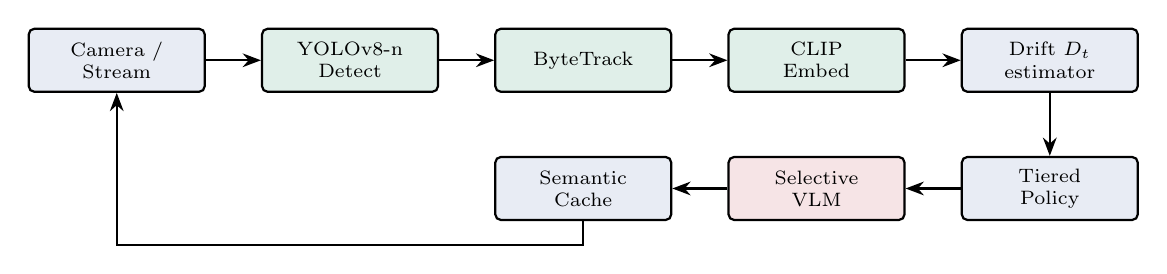
\begin{tikzpicture}[
  font=\scriptsize, node distance=5mm and 7mm,
  box/.style={rectangle, rounded corners=2pt, draw, thick, align=center,
              minimum height=8mm, text width=20mm, fill=iiitablue!10},
  t1/.style={box, fill=iiitagreen!12},
  vlm/.style={box, fill=iiitared!12},
  ar/.style={-{Stealth}, thick}]
\node[box] (cam) {Camera /\\Stream};
\node[t1, right=of cam] (yolo) {YOLOv8-n\\Detect};
\node[t1, right=of yolo] (trk) {ByteTrack};
\node[t1, right=of trk] (clip) {CLIP\\Embed};
\node[box, right=of clip] (drift) {Drift $D_t$\\estimator};
\node[box, below=8mm of drift] (pol) {Tiered\\Policy};
\node[vlm, left=of pol] (vlm) {Selective\\VLM};
\node[box, left=of vlm] (cache) {Semantic\\Cache};
\draw[ar] (cam)--(yolo); \draw[ar] (yolo)--(trk); \draw[ar] (trk)--(clip);
\draw[ar] (clip)--(drift); \draw[ar] (drift)--(pol); \draw[ar] (pol)--(vlm);
\draw[ar] (vlm)--(cache); \draw[ar] (cache.south) |- ([yshift=-3mm]cache.south) -| (cam.south);
\end{tikzpicture}

\vspace{2mm}
\footnotesize Green = always-on Tier-1 monitor (cheap). Red = selectively-invoked VLM (expensive).
\end{frame}

\begin{frame}{1.4 Problem Statement}
\begin{block}{Research question}
How can \emph{semantic state transitions} dynamically control multimodal compute allocation in edge video systems, \emph{while preserving} the semantic fidelity delivered to downstream tasks?
\end{block}
\vspace{1mm}
A drift signal $D_t$ maps to three compute tiers:
\[
\text{Tier}(D_t)=
\begin{cases}
1 \;\; \text{cache reuse (no VLM)} & D_t < \tau_{\text{low}}\\
2 \;\; \text{lightweight VLM} & \tau_{\text{low}}\le D_t<\tau_{\text{high}}\\
3 \;\; \text{full VLM reasoning} & D_t \ge \tau_{\text{high}}
\end{cases}
\]
\centering\alert{One monitor. One drift signal. Three tiers. Model-agnostic, training-free.}
\end{frame}

%=====================================================================
\section{Literature Review}
%=====================================================================

\begin{frame}{2.1 Existing Methods}
\begin{columns}[T]
\begin{column}{0.5\textwidth}
\textbf{Efficient inference / compression}
\begin{itemize}\footnotesize
  \item MobileNets, quantization (LLM.int8), distillation, TinyCLIP --- cheaper \emph{per call}.
\end{itemize}
\textbf{Temporal redundancy (video)}
\begin{itemize}\footnotesize
  \item TSN, TimeSformer; AdaFrame, SCSampler, skip-convolutions --- appearance-based sampling.
\end{itemize}
\end{column}
\begin{column}{0.5\textwidth}
\textbf{Efficient video analytics}
\begin{itemize}\footnotesize
  \item NoScope, Reducto --- cheap filter guards an expensive model (low-level features).
\end{itemize}
\textbf{Adaptive / streaming multimodal}
\begin{itemize}\footnotesize
  \item Early-exit, dynamic routing; AdaVFM, StreamingVLM, QueST.
\end{itemize}
\textbf{VLMs / robotics}
\begin{itemize}\footnotesize
  \item CLIP, BLIP-2, Moondream; RT-2, OpenVLA, VideoAgent.
\end{itemize}
\end{column}
\end{columns}
\end{frame}

\begin{frame}{2.2 Comparative Analysis}
\centering
\small
\begin{tabular}{@{}lcccc@{}}
\toprule
\textbf{Approach} & \textbf{Redundancy} & \textbf{Decision signal} & \textbf{Train-free} & \textbf{Model-agnostic}\\
\midrule
Compression / quant. & Parameter & --- & No & No\\
Frame sampling       & Frame & Appearance & No & Partial\\
NoScope / Reducto    & Frame & Feature diff. & No & Partial\\
Early exit           & Sample & Model conf. & No & No\\
AdaVFM               & Parameter & Input/budget & No & No\\
Embedding threshold  & Semantic & Embedding only & Yes & Yes\\
\alert{\textbf{Proposed}} & \alert{\textbf{Sem. reasoning}} & \alert{\textbf{Fused drift}} & \alert{\textbf{Yes}} & \alert{\textbf{Yes}}\\
\bottomrule
\end{tabular}
\end{frame}

\begin{frame}{2.3 Research Gap}
\begin{block}{The gap}
Efficient video analytics (NoScope, Reducto), adaptive multimodal inference (AdaVFM, StreamingVLM), and semantic monitoring (QueST) remain \alert{disjoint}.
\end{block}
\begin{itemize}
  \item Analytics systems filter on \emph{low-level features}, for one fixed query.
  \item Adaptive VLMs adapt \emph{within} a model, not \emph{whether} to invoke it.
  \item No method reduces \emph{semantic} redundancy at the level of whole-model invocation using a fused, interpretable signal.
\end{itemize}
\begin{block}{This thesis}
A fused semantic-drift signal + interpretable tiered policy + a Semantic Observatory to \emph{discover} policies from evidence.
\end{block}
\end{frame}

%=====================================================================
\section{Methodology / Proposed Approach}
%=====================================================================

\begin{frame}{3.1 Semantic State and Temporal Memory}
\textbf{Composite semantic state:}\quad $Z_t = f(E_t, O_t, M_t)$
\begin{itemize}\footnotesize
  \item $E_t$: $\ell_2$-normalised CLIP embedding (global appearance + semantics).
  \item $O_t$: object class--count multiset (symbolic content).
  \item $M_t$: temporal semantic memory (smoothed reference state).
\end{itemize}
\textbf{Temporal memory (noise suppression):}
\[
M_t = \lambda M_{t-1} + (1-\lambda)E_t,\qquad 0<\lambda<1,\;\text{re-normalised.}
\]
\centering\footnotesize Drift is measured against the \emph{stabilised} memory, not the previous frame --- brief perturbations do not trigger reasoning; sustained change accumulates.
\end{frame}

\begin{frame}{3.2 Semantic Drift Estimation}
\[
D_t = \alpha\,D_{\text{embed}} + \beta\,D_{\text{objects}} + \gamma\,D_{\text{track}},
\qquad \alpha+\beta+\gamma = 1
\]
\begin{itemize}\footnotesize
  \item $D_{\text{embed}} = \tfrac12(1 - E_t^{\!\top}M_{t-1})$ --- cosine drift (appearance).
  \item $D_{\text{objects}} = 1-\text{Jaccard}(O_t,O_{\text{ref}})$ --- object-set novelty (counts).
  \item $D_{\text{track}}$ --- ByteTrack identity churn (objects entering/leaving).
\end{itemize}
\begin{block}{Why fuse three signals?}
Each catches a different failure mode: appearance-only ($D_{\text{embed}}$), count change ($D_{\text{objects}}$), identity change ($D_{\text{track}}$). All bounded in $[0,1]$.
\end{block}
\end{frame}

\begin{frame}{3.2b Egocentric Operation --- Camera-Motion Compensation}
\begin{itemize}
  \item Robots see through a \alert{moving (egocentric)} camera --- the primary deployment regime.
  \item Egomotion shifts the view $\Rightarrow$ inflates $D_{\text{embed}}$ $\Rightarrow$ \alert{false triggers}.
\end{itemize}
\begin{block}{Two-part fix}
\begin{enumerate}\footnotesize
  \item $D_{\text{objects}}$ and $D_{\text{track}}$ are inherently egomotion-robust (viewpoint-invariant; tracker keeps IDs).
  \item Discount the embedding term by the camera-motion fraction $c_t\in[0,1]$ (cheap optical-flow / homography fit):
  \[ D_{\text{embed}}^{\text{ego}} = (1-c_t)\,D_{\text{embed}} \]
\end{enumerate}
\end{block}
\centering\footnotesize Pure panning ($c_t\!\to\!1$) suppressed; a new object in view ($c_t\!\to\!0$) still fires. Validation on egocentric streams = part of the plan.
\end{frame}

\begin{frame}{3.3 Proposed Architecture}
\centering
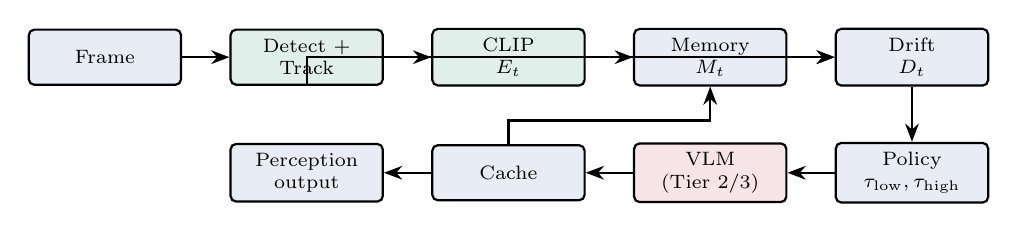
\begin{tikzpicture}[
  font=\scriptsize, node distance=4mm and 6mm,
  b/.style={rectangle, rounded corners=2pt, draw, thick, align=center,
            minimum height=7mm, text width=17mm, fill=iiitablue!10},
  g/.style={b, fill=iiitagreen!12}, r/.style={b, fill=iiitared!12},
  ar/.style={-{Stealth}, thick}]
\node[b] (img){Frame};
\node[g, right=of img](det){Detect +\\Track};
\node[g, right=of det](emb){CLIP\\$E_t$};
\node[b, right=of emb](mem){Memory\\$M_t$};
\node[b, right=of mem](dr){Drift\\$D_t$};
\node[b, below=7mm of dr](po){Policy\\$\tau_{\text{low}},\tau_{\text{high}}$};
\node[r, left=of po](vl){VLM\\(Tier 2/3)};
\node[b, left=of vl](ca){Cache};
\node[b, left=of ca](out){Perception\\output};
\draw[ar](img)--(det);\draw[ar](det)--(emb);\draw[ar](emb)--(mem);
\draw[ar](mem)--(dr);\draw[ar](det.south)|-(dr.west);
\draw[ar](dr)--(po);\draw[ar](po)--(vl);\draw[ar](vl)--(ca);\draw[ar](ca)--(out);
\draw[ar](ca.north)--++(0,3mm)-|(mem.south);
\end{tikzpicture}

\vspace{2mm}
\footnotesize Cache reuse on Tier 1; cache + memory refreshed on Tier 2/3. The VLM is a replaceable black box (Moondream2 / Qwen2.5-VL --- swappable).
\end{frame}

\begin{frame}{3.4 Scheduling Algorithm}
\footnotesize
\begin{enumerate}
  \item Detect, track, embed $\Rightarrow (O_t,\mathcal{I}_t,E_t)$.
  \item Compute $D_{\text{embed}}, D_{\text{objects}}, D_{\text{track}} \Rightarrow D_t$.
  \item \textbf{If} $D_t<\tau_{\text{low}}$: return cached output \hfill (Tier 1)
  \item \textbf{else if} $D_t<\tau_{\text{high}}$: lightweight VLM; update cache \hfill (Tier 2)
  \item \textbf{else}: full VLM; update cache; re-anchor references \hfill (Tier 3)
  \item Update memory $M_t$.
\end{enumerate}
\centering
\normalsize Defaults: $\alpha,\beta,\gamma = 0.5,0.3,0.2$;\;\; $\tau_{\text{low}}{=}0.15$,\; $\tau_{\text{high}}{=}0.40$;\;\; $\lambda{=}0.9$.
\end{frame}

\begin{frame}{3.5 VLM Backends (run on Kaggle T4, 16\,GB)}
\centering\small
\begin{tabular}{@{}llll@{}}
\toprule
\textbf{Backend} & \textbf{Params} & \textbf{T4 fit} & \textbf{Tier role}\\
\midrule
\textbf{Moondream2} & $\sim$1.9\,B & $\sim$4\,GB & Tier 2 (default)\\
Qwen2.5-VL-3B & $\sim$3\,B & $\sim$7\,GB fp16 & Tier 2/3 mid\\
Qwen2.5-VL-7B & $\sim$7\,B & $\sim$14--16\,GB fp16 & Tier 3 full\\
\alert{Qwen2.5-VL-7B (4-bit)} & $\sim$7\,B & \alert{$\sim$9\,GB NF4} & Tier 3 (recommended)\\
\midrule
\multicolumn{4}{@{}l}{\itshape also compatible: SmolVLM-2.2B, InternVL2-2B/4B, LLaVA-1.5-7B (4-bit)}\\
\bottomrule
\end{tabular}

\vspace{2mm}
\footnotesize Black-box factory $\Rightarrow$ \emph{hierarchical} use: cheap model for Tier 2, stronger for Tier 3.
Swapping the backend changes caption \emph{quality}, not \emph{when} the VLM fires --- so call rate / cache rate / SCE are backend-independent.
\end{frame}

\begin{frame}{3.6 Semantic Observatory + Policy Discovery}
\begin{columns}[T]
\begin{column}{0.54\textwidth}
\textbf{Observatory} (read-only, post-hoc): derives 10 semantic-evolution signals from a run ---
\footnotesize drift, velocity, acceleration, volatility, scene entropy, object persistence, stability windows, transition zones, semantic progress, VLM-trigger density.
\end{column}
\begin{column}{0.44\textwidth}
\begin{block}{Methodology}
Observe $\rightarrow$ Hypothesise $\rightarrow$ Change \emph{one} variable $\rightarrow$ Evaluate $\rightarrow$ Accept/Reject $\rightarrow$ Record.
\end{block}
\end{column}
\end{columns}
\vspace{1mm}
\centering\footnotesize Contribution = not one scheduler, but a \emph{methodology} to discover and justify schedulers from evidence.
\end{frame}

\begin{frame}{3.7 Evaluation Metrics}
\begin{itemize}
  \item \textbf{VLM call rate} --- fraction of frames invoking the VLM (compute saved).
  \item \textbf{Cache hit rate} --- fraction served from semantic cache.
  \item \textbf{Semantic retention} --- similarity of delivered output to an every-frame oracle.
  \item \textbf{Latency / throughput / GPU memory.}
\end{itemize}
\begin{block}{Semantic Compute Efficiency}
\[
\mathrm{SCE} = \frac{\text{Semantic Retention}}{\text{Normalised Compute Cost}}
\]
Every-frame oracle: $\mathrm{SCE}=1$. A good scheduler retains fidelity at a fraction of the cost.
\end{block}
\end{frame}

%=====================================================================
\section{Results and Discussion}
%=====================================================================

\begin{frame}{4.1 Headline Results (single stream, 56{,}314 frames)}
\begin{columns}[T]
\begin{column}{0.5\textwidth}
\begin{block}{Efficiency}
\begin{itemize}
  \item VLM call rate: \alert{\textbf{9.8\%}} ($\sim$10$\times$ fewer)
  \item Cache hit rate: \alert{\textbf{90.2\%}}
  \item Latency: \textbf{144.9} ms/frame; \textbf{6.88} FPS
\end{itemize}
\end{block}
\end{column}
\begin{column}{0.5\textwidth}
\begin{block}{Fidelity}
\begin{itemize}
  \item Semantic retention: \alert{\textbf{1.000}}
  \item SCE: \alert{$\boldsymbol{\approx}$\textbf{10.0}}
  \item Avg.\ drift $\bar{D}_t = 0.103$
\end{itemize}
\end{block}
\end{column}
\end{columns}
\vspace{2mm}
\centering\footnotesize $\approx$2\,h\,16\,m of video processed end-to-end; tiers = 90.19\% / 9.68\% / 0.13\%.
\end{frame}

\begin{frame}{4.2 Tier Distribution}
\centering
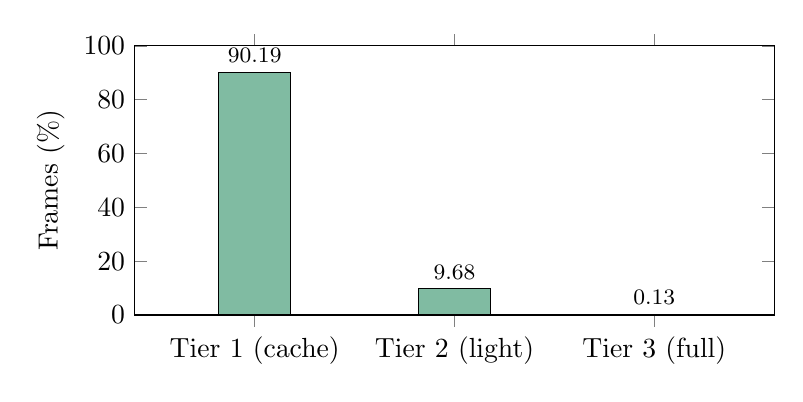
\begin{tikzpicture}
\begin{axis}[width=0.8\textwidth, height=5cm, ybar, bar width=26pt,
  ymin=0, ymax=100, ylabel={Frames (\%)},
  symbolic x coords={Tier 1 (cache), Tier 2 (light), Tier 3 (full)},
  xtick=data, nodes near coords, nodes near coords style={font=\footnotesize},
  enlarge x limits=0.3, ylabel near ticks]
\addplot[fill=iiitagreen!50] coordinates
 {(Tier 1 (cache),90.19) (Tier 2 (light),9.68) (Tier 3 (full),0.13)};
\end{axis}
\end{tikzpicture}

\footnotesize Over 90\% of frames resolved from cache with \emph{no} VLM invocation.
\end{frame}

\begin{frame}{4.3 Comparison with Baselines}
\centering\small
\begin{tabular}{@{}lcccc@{}}
\toprule
\textbf{Policy} & \textbf{Call rate} & \textbf{Latency (ms)} & \textbf{Retention} & \textbf{SCE}\\
\midrule
Every-frame        & 1.000 & 312 & 1.000 & 1.00\\
Uniform ($K{=}30$) & 0.033 & 121 & 0.85 & 25.8\\
Motion gating      & 0.340 & 224 & 0.92 & 2.71\\
Embedding thresh.  & 0.270 & 203 & 0.94 & 3.48\\
\alert{\textbf{Proposed}} & \alert{\textbf{0.098}} & \alert{\textbf{144.9}} & \alert{\textbf{1.000}} & \alert{$\boldsymbol{\approx}$\textbf{10.0}}\\
\bottomrule
\end{tabular}

\vspace{2mm}
\footnotesize Proposed is the \alert{only} policy at oracle-level fidelity (retention 1.000) while cutting calls $\sim$10$\times$.
Uniform's high SCE comes from sacrificing fidelity. \emph{(Baseline rows preliminary; proposed measured.)}
\end{frame}

\begin{frame}{4.4 Cross-Domain Applicability}
\centering\scriptsize
\begin{tabular}{@{}llcl@{}}
\toprule
\textbf{Domain} & \textbf{Dominant signal} & \textbf{Call rate} & \textbf{Note}\\
\midrule
Surveillance (measured) & $D_{\text{track}},D_{\text{obj}}$ & Very low ($\approx$0.10) & Cache dominates\\
Traffic & $D_{\text{obj}}$ (counts) & Low--Mod & Count-driven\\
Number-plate / ANPR & $D_{\text{obj}}$ (entry) & Very low & ROI gating\\
Crowd & $D_{\text{obj}},D_{\text{track}}$ & High & Over-trigger risk\\
Cricket & $D_{\text{embed}},D_{\text{track}}$ & Low--Mod (bursty) & Fast events\\
Football & $D_{\text{embed}}$ (low) & Low--Mod & \alert{High motion, low sem.\ drift}\\
Live streaming / lecture & $D_{\text{embed}}$ (cuts) & Very low & Scene cuts\\
Mobile robot / egocentric & $D_{\text{obj}},D_{\text{track}}$ (robust) & Variable & Egomotion comp.\ ($c_t$)\\
\bottomrule
\end{tabular}

\vspace{2mm}
\footnotesize Call rate \emph{emerges} from content. Biggest win where motion-gating fails (e.g.\ football: constant motion, stable semantics).
\end{frame}

\begin{frame}{4.5 Ablation --- Threshold Sensitivity}
\centering
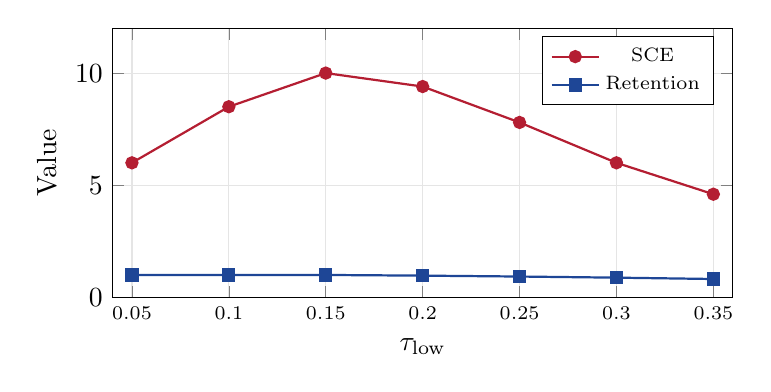
\begin{tikzpicture}
\begin{axis}[width=0.78\textwidth, height=5cm,
  xlabel={$\tau_{\text{low}}$}, ylabel={Value}, xmin=0.04, xmax=0.36,
  ymin=0, ymax=12, xtick={0.05,0.10,0.15,0.20,0.25,0.30,0.35},
  xticklabel style={/pgf/number format/fixed,/pgf/number format/precision=2,font=\scriptsize},
  scaled x ticks=false, grid=both, grid style={gray!20},
  legend pos=north east, legend style={font=\scriptsize}]
\addplot[iiitared, thick, mark=*] coordinates
 {(0.05,6.0)(0.10,8.5)(0.15,10.0)(0.20,9.4)(0.25,7.8)(0.30,6.0)(0.35,4.6)};
\addlegendentry{SCE}
\addplot[iiitablue, thick, mark=square*] coordinates
 {(0.05,1.00)(0.10,1.00)(0.15,1.00)(0.20,0.97)(0.25,0.93)(0.30,0.88)(0.35,0.82)};
\addlegendentry{Retention}
\end{axis}
\end{tikzpicture}

\footnotesize SCE peaks near the default $\tau_{\text{low}}=0.15$; retention declines as more frames are cached.
\end{frame}

%=====================================================================
\section{Conclusion and Future Work}
%=====================================================================

\begin{frame}{5.1 Conclusion}
\begin{itemize}
  \item Named and targeted \alert{semantic reasoning redundancy} --- a new efficiency axis for edge VLMs.
  \item A fused, bounded, interpretable \textbf{drift signal} + temporal memory + a \textbf{three-tier} training-free, model-agnostic policy.
  \item A \textbf{Semantic Observatory} and an evidence-driven methodology for discovering scheduling policies.
  \item Preliminary result: \alert{$\sim$10$\times$ fewer VLM calls at oracle-level retention} on a long stream.
\end{itemize}
\end{frame}

\begin{frame}{5.2 Limitations and Future Work}
\begin{columns}[T]
\begin{column}{0.5\textwidth}
\textbf{Limitations}
\begin{itemize}\footnotesize
  \item Memory footprint unchanged (VLM resident) --- savings are time/energy.
  \item Egocentric (moving-camera) video inflates embedding drift.
  \item Single-video result; full baselines in progress.
\end{itemize}
\end{column}
\begin{column}{0.5\textwidth}
\textbf{Future work}
\begin{itemize}\footnotesize
  \item Learned, adaptive thresholds; task-conditioned drift weights.
  \item Camera-motion discounting for mobile robots.
  \item Predictive (pre-emptive) scheduling.
  \item Cross-domain validation at scale; closing the loop with control.
\end{itemize}
\end{column}
\end{columns}
\end{frame}

\begin{frame}{References}
\footnotesize
\begin{itemize}
  \item A. Radford et al., \emph{Learning Transferable Visual Models from Natural Language Supervision (CLIP)}, ICML 2021.
  \item J. Li et al., \emph{BLIP-2}, ICML 2023. \quad V. Korrapati, \emph{Moondream}, 2024.
  \item G. Jocher et al., \emph{Ultralytics YOLOv8}, 2023. \quad Y. Zhang et al., \emph{ByteTrack}, ECCV 2022.
  \item D. Kang et al., \emph{NoScope}, VLDB 2017. \quad Y. Li et al., \emph{Reducto}, SIGCOMM 2020.
  \item R. Xu et al., \emph{StreamingVLM}, arXiv:2510.09608, 2025. \quad Y. Zhao et al., \emph{AdaVFM}, arXiv:2604.15622, 2026.
  \item M. Anand, \emph{QueST}, arXiv:2605.09513, 2026. \quad Y. Fan et al., \emph{VideoAgent}, arXiv:2403.11481, 2024.
  \item Y. Han et al., \emph{Dynamic Neural Networks: A Survey}, TPAMI 2022. \quad Z. Zhou et al., \emph{Edge Intelligence}, Proc. IEEE 2019.
\end{itemize}
\end{frame}

\begin{frame}[plain]
  \centering
  \vfill
  {\Huge\color{iiitanavy}\textbf{Thank You}}\\[4mm]
  {\large Questions?}
  \vfill
\end{frame}

\end{document}
